\chapter{Implementation}\label{ch:problem}
\section{Breaking Down the Problem}
Having examined the state of art developments of \gls{SSGPVS}, what are essentials to successfully make a \gls{SSGPVS} using \gls{RT} simulators and microcontroller is pretty clear. Although theory behind \gls{SSGPVS}  has been studied for quite a long time and there has been existing products on the market already, documentations on development process of a \gls{RT} or \gls{HIL} simulation are still limited. So far the reviews have shed the light on tasks needed to complete the whole project. 

The first task is to develop a \gls{SSGPVS} in the pure software environment which may pave th way for developing a \gls{RT} model for the simulator. The process involved is described in detail in \Vref{sec:build_simulink}. The second issue which is discussed in \Vref{sec:convert_rt} is to revise the model so that it can be load into \gls{RT} simulator and runs in \gls{RT}. 
The third issue is to implement the controller functionalities using a \gls{DSP}. The implementation involves some advanced C language programing which is something I enjoy doing. The details of implementation are presented in \Vref{sec:implement_micro}.
The fourth issue which discussed in \Vref{sec:perform_pil} is to perform \gls{PIL} simulation. This issue is a little bit complicated since it requires me to be well familiar with the real time simulator. And I have not found much resources on this so far. It is a milestone to this project.
\section{Building Model in SIMULINK}\label{sec:build_simulink}
The purpose of a pure software simulation model is to verify the correctness of circuit topology, solar panel model and proper design of LCL filter. Luckily, SIMULINK has a build-in \gls{SSGPVS} model which can be found in \textit{MALTAB 2015B} and later versions\cite{solar_buildin_model}. It provide a good starting point of this project. Since the project focus on performing \gls{RT} simulations, any already known to work model can be used to accelerate the process of building the whole model and save some time avoid doing everything from scratch. 

The model was quite well designed and simulation ran with not error. Minor adjustment may be made before turning it into a \gls{RT} model. The system was design for North America market which result in a 60 Hz operation of grid frequency. Since the grid voltage in Australia is 50 Hz, the grid frequency of original model need to be change to 50 Hz. In order to change the frequency, the minimum time step, \gls{PWM} frequency of the inverter and controller sampling time need to be changed as well. The reason for changing the minimum time step is that fixed time solver for solving ordinary differential equations(ODE) is used for simulation which means grid frequency, controller sampling time or any other components' sampling time need to be integer multiple of minimum time step. \Vref{tab:change_list} is a summary of different configurations between models. 
\begin{center}\label{tab:change_list}
\begin{tabular}{ |c|c|c| } 
 \hline
 Items Changed & Origin Configuration & New Configuration\\ \hline
 Minimum time step &  $1.323e^{-6}$ s & $6.25e^{-7}$ s \\ \hline
 Carrier frequency & 3780 Hz & 8000 Hz\\ \hline
 Controller sampling & $2.6455e^{-5}$ s& $1.25e^{-5}$ s\\ \hline
\end{tabular}
\end{center}

Noticing that the switching frequency is set to 8 kHz because higher switching frequency may lead to less bulky inductors in real life which is less expensive. Instead of setting switching frequency to nearer 4 kHz, double of the frequency is chosen. In order to ensure the accuracy of simulation and avoid limited resolution on duty cycle, $6.25e^{-7}$ s of minimum time step has been chosen to ensure minimum stepping of duty cycle is 0.5\%. The duty cycle resolution could affect \gls{SSGPVC} creating high output current THD and undesired phase shift since duty cycle can only vary in discrete steps.

Changed made in \gls{PWM} frequency lead to smaller minimum time step, thus, more time needed to generate one second simulation results. The time it takes to run the simulation depends on configurations of the host PC and it is common to run simulation for around five minutes to generate one second of results. 

The controller design in the model is different from what has been mentioned previously. Bearing in mind that the purpose of using this model is to obtain a working plant for performing \gls{RT} simulation in the next stage, as a result, the design of the controller is not thoroughly studied. 

\section{Convert to Real-time}\label{sec:convert_rt}
After getting a working model running in SIMULINK, the model should be convert to \textit{RTLAB} compatible model. Currently, \textit{RTLAB} only support \textit{MATLAB 2014B}, the first thing to do is to make sure the model can still work under \textit{2014B}. Unfortunately, the model makes use of a generic solar \gls{PV} model which is only rendered in \textit{2015B}. In order to continue doing simulation, the \gls{PV} model need to be replaced with a replica.

\subsection{Custom Solar Cell}
Since access to source code to \textit{MALTAB}'s PV panel model is not possible, creating a replica of the \textit{MALTAB}'s model is important so that it would be possible to verify the custom solar cell model is acutally correctly implemented. Based on what has been stated in \Vref{sec:solar_cell}, the custom model was initially built up in a script in \textit{MALTAB}. Since scripts or functions written in \textit{MATLAB} is also compatible to run using SIMULINK, it should not be difficult to integrate the script into existing \gls{SSGPVS} model. 

The initial idea was to implement a generic \gls{PV} cell which only relies on some key parameters that represent the external characteristic of the cell. The parameters include open circuit voltage, short circuit current and temperature coefficients of voltage/current. As for the internal serial and parallel connected resistors, they may be obtained via proper calculation. In this way, the model can be easily extended to simulate any cell or panel of interest. However, how to archive this goal is not clear at the time when the model was implemented since the resistors' value are usually acquired via measurements made by the manufacturers of of the cell/panel. Not many article which is available shed light on how to accurately estimate those parameters from external characteristic of cell/panel, which makes it difficult to fulfill this goal. As a workaround, the model was implemented under the condition that the two parameters are provided by the manufacturer, otherwise there is no way to implement the model. 

The first version of the cell model was implemented as a completely standalone model (black box) which does not reply on any \simulink~ models. The first trial was based on \cite{RN26} since the model it proposed is simple and easy to understand. However, the model in the article is a simplified one which shunt resister is not considered. Also, Newton's method was used to derive serial resistor value of the cell, of which is based on iteration. Newton's method may fail to converging to local minimum point when variables are trapped in saddle points. 
\cite{RN24} has more details on models which have different levels of simplification and equations are well presented. This makes it easier to understand and implement the model. Model presented in \cite{RN24} were built-in native \simulink~, however, using 'drag and drop' method has limitation on the maximum efficiency that one can archive. That's the reason that custom model implemented in this project is written as a script and the running results are presented in the later chapter.

It turned out that the idea to make the model as a black box is not a good idea because this approach makes it hard to interface with the rest of the system in \simulink~~. Interestingly, \simulink~~'s way of modeling a circuit system is different from doing numerical calculations. It is not possible to directly interface circuit models with numerical calculation blocks. Custom components need to be implemented using controlled voltage or current source. Considering the design rules imposed by \simulink~~, there is no choice but to implement custom model partially based on \simulink~~ native blocks (mainly controlled sources) to reuse most of work has been finished before. 
\begin{figure}[h]
     \centering
     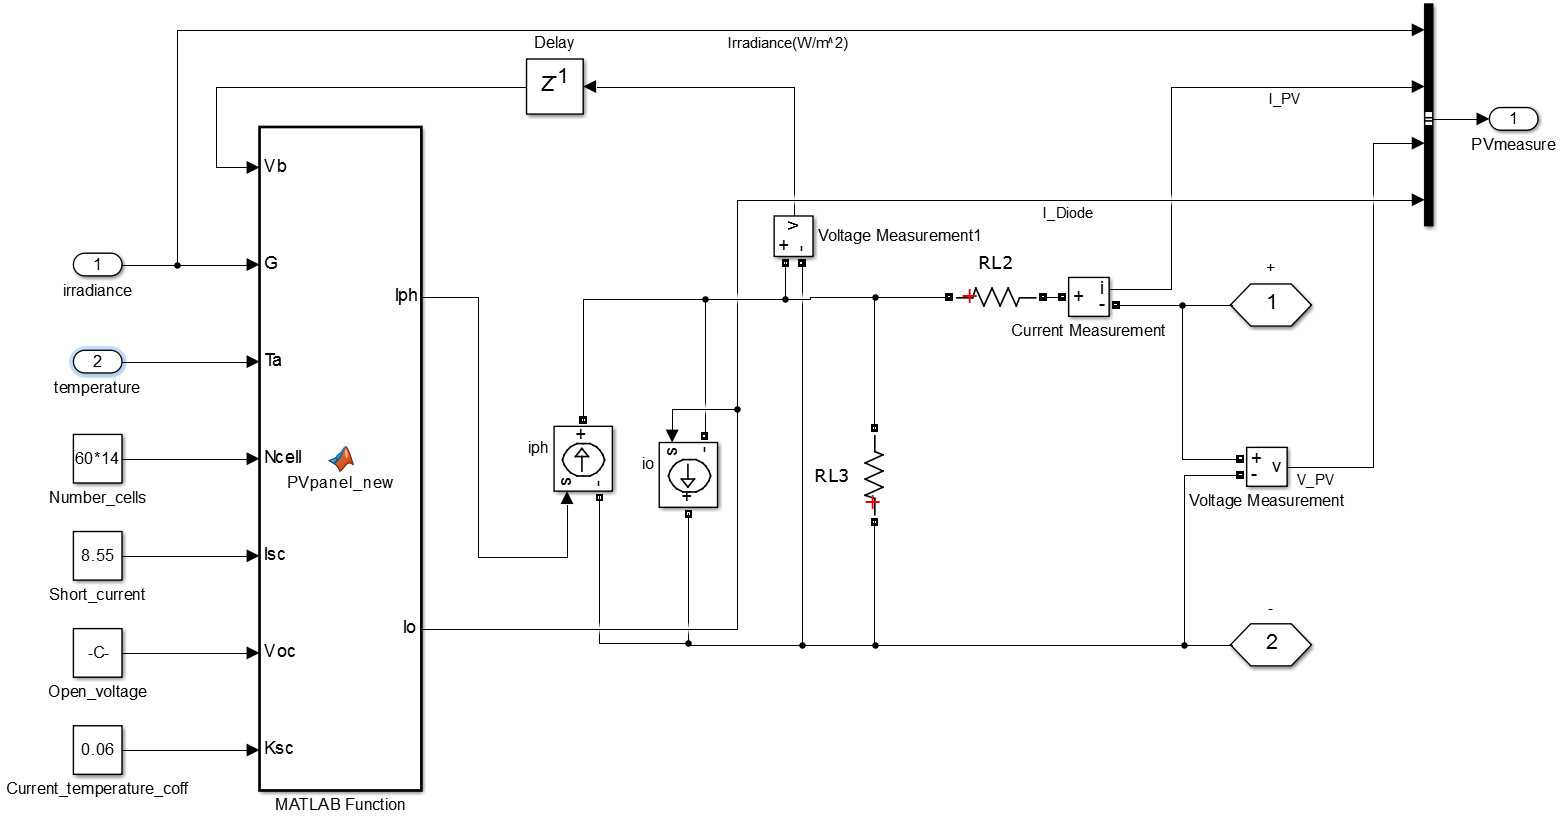
\includegraphics[width = 1\textwidth]{figures/custome_pv}
     \caption{Custom solar cell model}
     \label{fig:cell_model}
\end{figure}

\Vref{fig:cell_model} illustrates the final version of custom solar cell model and it is a replica of model that used before. Algebraic loop which is often the reason why simulation cannot run is a critical issue encountered during the process of making the model. Examining Equation \ref{equ:solar cell} carefully, it is not hard to find that output current of solar cell depends on terminal voltage of the cell. The terminal voltage, in turn, depends on output current flow through external load. This means that in order to calculate either of them, at least one parameter has already been known,  which forms a classic algebraic loop. For the sake of running simulation, algebraic loop need to be broken by introducing delays into the system. The presence of a delay module in \Vref{fig:cell_model} is to break algebraic loop and setting up initial condition properly. Sometimes, extra delay may lead to unstable operation of the system, however, it is not a problem with custom model fortunately.

\subsection{RTLAB}
As menstioned before, \gls{RT} model should be able to run using RTLAB because RTLAB is the only software that is capable of communicate with Opal-RT's simulators. The workflow to work with RTLAB is listed below. 
\begin{enumerate}
\item \textbf{Create a new project} \\
New project should be created with human readable project name. This would create a new folder to hold all the project related files including \gls{RT} models and configurations and completions. 
\item \textbf{Import exisitng model} \\
Two options are available during this stage, one is template model provided by the Opal-RT, the other one is directly import the known to work model created previously. For a brand new pure software model, it is recommended  to import the templates, then copy the pure software model into the template. In this way, users do not need to configure all the settings from scratch, however, caution need to be taken because some configurations may not be suitable for any models. 
\item \textbf{Moidify model} \\
Once imported, users should be able to edit the model via \rtlab~ launched \matlab~ window. There are some requirements imposed by \rtlab~ and users need to make sure the model should be able to compile and run offline (without loading onto simulator). Since \rtlab~ is not smart enough at the moment, it needs users' help to separating model into different functional blocks so that each functional blocks can use one processing core in the simulator to maximize performance by running simulation in parallel. Different cores may communicate with each other synchronously or asynchronously depends on users' preference. 
\item \textbf{Build \gls{RT} model} \\
The reason for this step is that simulator cannot run \matlab~ model directly (and should not). In fact, \simulink~ as a high level development environment, has relatively low efficiency running time critical simulation. However, with the help of \matlab~ coder, \simulink~ models can be compile into C/C++ which is a low level language that can be run of high efficiency. Generated files are stored in the project folder and once all completions are ready users may continue. 
\item \textbf{Load model and perform \gls{RT} simulation} \\
In this stage, all completions are transferred from host PC to simulator and \rtlab~ would put simulator into ready state. Once users click on button to start simulation, simulator would start running and user may use auto-generated console window to interact directly with the simulator. Users may choose to pause or stop simulation at anytime via \rtlab.
\end{enumerate}
\subsection{\ehs}
\ehs is a generic and reconfigurable FPGA-based electrical solver which provides a convenient user interface enabling users to bring into \gls{RT}models created in the simulation tool of different mainstream simulation environment including \simulink, PSIM, PLECS Blockset, and Multisim. \ehs operate at a much finer time resolution, so communication between \ehs and \gls{CPU} cores is archived by sampling. At the beginning of each calculation, \ehs solver samples the values in \gls{CPU} and perform calculations based on the sampled values. 

In \simulink, \ehs solver is represented as a block diagram and it contains many parameters that users may like to change. Here are some differences between building a regular \rtlab~ model and \ehs model.
\begin{enumerate}
\item \textbf{Separate model into two files} \\
\rtlab~ allows users to put models from \textit{SimScape Power System \simulink~ toolbox} together with normal numerical calculation block under the same subsystem. The idea behind separation of simulation file is still the same. Because \rtlab~ and \ehs are not that smart, they need manual process of separation. Briefly, \ehs is able to handle majority of circuit models in \textit{SimScape Power System toolbox}. Instead of separate those models into subsystem under the same file, they need to be separated into two different files.  The rest of the system, apart from those power system models, become master of model and interface with power system models with \ehs block diagram. 
\item \textbf{Changing naming of used power system models} \\
\ehs makes use of pre-generated \gls{FPGA} firmware that have special requirements on naming of each modules used in simulation model. By following the naming convention, model translator is able to map each modules onto different sections of digital circuit that take advantage of parallel computation power rendered by \gls{FPGA}. 
\end{enumerate}
\section{Implementation In Microcontroller}\label{sec:implement_micro}
\begin{figure}[h]
     \centering
     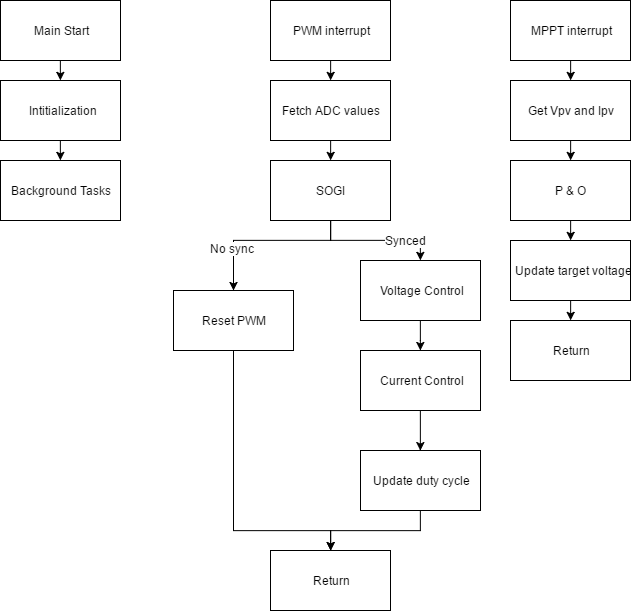
\includegraphics[width = 1\textwidth]{figures/software_flow}
     \caption{Software flowchat}
     \label{fig:software_flow}
\end{figure}
\Vref{fig:software_flow} illustrates software flow implemented in TMS320F28027(F28027). Since objective of this project is to implement a simple \gls{SSGPVS} and perform \gls{HIL} simulation to prove the concept of fast prototyping and development without real hardware, only the necessary elements are implemented in the \tms. 
\subsection{IQ math}
Due to the fact that our microcontroller is a fixed point microcontroller, there is no floating point processing in \tms. We cannot execute any floating point arithmetic using \tms, however, it is still possible to use float point numbers when writing codes. Compiler has the ability to handle the situation to perform float point calculations using software implemented floating point library. The performance is largely sacrificed because what the software floating point library does is to calculate floating numbers using \fp~ using iterative numerical methods. Depends on implementation of software library, multiplications on microcontroller might take so long that in hard \gls{RT} applications program can fail to meet computational deadline. Especially for digital control of power electronic applications, modern designs call for higher and higher \gls{PWM} frequency in order to minimize size of passive components, thus, increased bandwidth requirements for controllers. 

Fortunately, \tms~ has 32x32 and 16x16 Multiply-accumulate(MAC) units inside that offer possibilities to do multiplication using less than 10 clock cycles, which make it promising for \gls{SSGPVS} applications with a reasonable \gls{PWM} frequency. In order to make use of MAC, software developers need to code in assembly because compiler might not be able to directly translate \fp~ multiplications into assembly efficiently. to squeeze every possible improvement on performance. Usually development in assembly is extremely time consuming and violate origin purpose of fast prototyping. Texas Instruments provides IQ math library as a solution to avoid dilemmas like this. Using the library can ensure that all multiplications can make the most of MAC available. The following table has some key math operations and their benchmarks\cite{iqmath_lib} which are used intensively in the program.
\section{Performing \gls{PIL} Simulation}\label{sec:perform_pil}